\documentclass{article}
\pdfpagewidth=8.5in
\pdfpageheight=11in
% The file ijcai19.sty is NOT the same than previous years'
\usepackage{ijcai19}

%% your usepackages here, for example:
\usepackage{booktabs}

%% the rest of your preamble here
\usepackage{color}

\usepackage{bbm}
\usepackage{float}
\usepackage{amsmath}
\usepackage{todonotes}
\usepackage[linesnumbered,ruled,vlined]{algorithm2e}
\DeclareMathOperator*{\argmax}{arg\,max}
\DeclareMathOperator*{\argmin}{arg\,min}

%%Added
\usepackage{graphicx}
\usepackage{subcaption}
\usepackage{bbm}
\usepackage{hyperref}
\usepackage{amsfonts}
\usepackage{multirow}

\title{Exploring Computational User Models for Agent Policy Summarization}

\author{
Isaac Lage\footnote{Equal contribution}$^1$\and
Daphna Lifschitz$^*$$^2$\and
Finale Doshi-Velez$^1$\And
Ofra Amir$^2$\\
\affiliations
$^1$Harvard University\\
$^2$Technion - Israel Institute of Technology
\emails
isaaclage@g.harvard.edu,
daphna.l@campus.technion.ac.il,
finale@seas.harvard.edu,
oamir@technion.ac.il
}

\begin{document}

\maketitle

\begin{abstract}
AI agents are being developed to support high stakes decision-making processes from driving cars to prescribing drugs, making it increasingly important for human users to understand their behavior. Policy summarization methods aim to convey strengths and weaknesses of such agents by demonstrating their behavior in a subset of informative states. Some policy summarization methods extract a summary that optimizes the ability to reconstruct the agent's policy under the assumption that users will deploy inverse reinforcement learning. In this paper, we explore the use of different models for extracting summaries. We introduce an imitation learning-based approach to policy summarization; we demonstrate through computational simulations that a mismatch between the model used to extract a summary and the model used to reconstruct the policy results in worse reconstruction quality; and we demonstrate through a human-subject study that people use different models to reconstruct policies in different contexts, and that matching the summary extraction model to these can improve performance. Together, our results suggest that it is important to carefully consider user models in policy summarization.
\end{abstract}

\maketitle

\section{Introduction}
Autonomous and semi-autonomous agents are being developed and deployed to complete complex tasks such as driving or recommending clinical treatment. As these agents take a growing role in our daily lives, it is becoming increasingly important to provide ways for people to understand and anticipate their behavior. Recent works in the area of interpretability and explainable AI have thus developed methods for describing and explaining the decisions of agents to human users. A rich body of research focuses on explaining a \emph{specific} decision made by an agent to a human user. A recent complementary line of work focuses on \emph{summarizing} the \emph{global} behavior of the agent by demonstrating actions taken by the agent in different states~\cite{amir2018agent}. Such summaries have been shown to improve people's ability to assess agents' capabilities~\cite{amir2018highlights,huang2018establishing}, anticipate agents' actions~\cite{huang17communicate} and facilitate trust~\cite{huang2018establishing}. 

The problem of policy summarization, or extracting subsets of state-action pairs that globally characterize the agent's behavior, has been approached in two ways. The first approach applies heuristics related to the diversity or importance of states to determine what is shown in the summary~\cite{amir2018highlights,huang2018establishing}. The second approach assumes a computational model of how humans will generalize from the summaries provided, and uses that model to optimize the summary for reconstructing the agent's full policy \cite{huang17communicate}. Specifically, \cite{huang17communicate} assumed that people would deploy inverse reinforcement learning (IRL) to infer the agent's reward function from the summary; their summaries were created to perform well given this assumption of human computation. The cognitive science literature provides evidence that people sometimes do build models of others' behavior in this way~\cite{baker2009action,baker2011bayesian}, making IRL a plausible model. However, there also exists evidence that human planners sometimes rely on a model-free system that computes actions based on previous experience in a situation~\cite{daw2005arbitration}. People may do something similar when inferring the behavior of others, making imitation learning (IL) another plausible model of human computation. 

In this paper, we explore the effects of using different models for summary extraction on the ability to reconstruct a policy. We make the following contributions: (1) we develop an IL-based summary extraction method; (2) Through computational simulations in a variety of domains, we demonstrate that the model used during summarization needs to match the model used to reconstruct the policy to produce high quality reconstructions; and (3) we demonstrate through human-subject studies that people may deploy different models in different contexts and that in some cases matching summary extraction to reconstruction model results in improved policy reconstruction. Taken together, these results suggest the importance of carefully considering which computational models of users we employ during policy summarization.

\section{Related Work}

\textbf{Summarizing Agent Policies.} Policy summarization is the problem of extracting a collection of state-action pairs that globally characterize an agent's policy with the goal of helping a  user  understand it~\cite{amir2018agent}. One approach relies on heuristics based on agent Q-values and state similarity, to extract diverse, important states~\cite{amir2018highlights,huang2018establishing}. A second approach formalizes the problem through machine teaching, where the goal is to extract state-action pairs useful for recovering the agent's reward function with IRL~\cite{huang17communicate}. Our work extends the latter approach by additionally considering IL.

\textbf{Cognitive Science of Inferring Agent Behavior.}
\cite{dragan2014familiarization} show that people can learn to anticipate agent actions if they see enough examples, but some agent behaviors can never be fully anticipated. Baker et al.~\shortcite{baker2009action,baker2011bayesian} suggest that people use ``theory of mind'' to infer others' beliefs and desires based on observations of their actions, modeling people's inference as Bayesian inverse planning. \cite{daw2005arbitration} describes how human planning uses both a model-based system that computes rewards and transitions, and a model-free system that computes actions based on previous experience. While in their setting people learn by directly interacting with the world, a similar set of approaches may also be used when inferring actions of others. Work on agents modeling agents \cite{albrecht2018modeling} describes strategies including case-based reasoning, of which IL is an example, and utility reconstruction, of which IRL is an example. Finally, \cite{medin19778context} discusses the exemplar theory of classification in psychology that says that humans categorize new objects based on similarity to objects in their memory, motivating our choice of IL model.

\textbf{Explaining Agent Decisions.}
More broadly, our work relates to the area of explainable AI~\cite{aha2017ijcai}. Many approaches focus on explaining a specific decision \cite{khan2009minimal,lomas2012explaining,dodson2011natural,broekens2010explain} or showing which features the agent attends to~\cite{greydanus2017visualizing}. \cite{miller2018explanation} reviews findings from the social sciences regarding useful explanations, and defines an explanation as causal, providing an answer to a why-question. In contrast to these approaches, we consider a complimentary non-causal \emph{description} of the agent's global behavior. Closer to our work, \cite{vanderwaa2018contrastive} explains policies in terms of differences in expected outcomes from a user specified, contrast policy, and \cite{ramakrishnan2018blindspot} formalizes the problem of detecting ``blind spots'', situations in which an agent acts incorrectly because it cannot differentiate between important real world states. Our work aims to more generally provide a summary that highlights the agent's strengths as well as weaknesses without requiring the user to be able to specify a specific contrast.

\section{Methods}
\label{sec:methods}

Following \cite{huang17communicate}, we formalize the problem of extracting a summary of an agent's behavior as an instance of machine teaching, which aims to find a set of training examples that induces a known target model to learn a pre-specified source model~\cite{zhu2015machine}. In our setting, the agent's policy is the source model that we want to induce, and the target models that we consider are hypotheses about how humans generalize from examples of an agent's behavior---IRL and IL.
 
Formally, our problem is to find the set of examples $T$ of size $k$, where $T = \langle \langle s_{1},a_{1} \rangle,...,\langle s_{k},a_{k} \rangle \rangle$ is the set of state-action pairs that maximizes the similarity $\rho$ of the policy induced by $T$ under a specific target computational model $M$. The objective can be written as:
\begin{equation}
 \max_{T \in \mathcal{D}} \rho( \hat{\pi}(T,M), \pi^*)\\
 \texttt{s.t.} |T| = k
\end{equation}
where $\mathcal{D}$ is all state-action pairs demonstrating the agent's policy, $\pi^{*}$, $\hat{\pi}(T,M)$ is the approximate policy attained by applying computational model $M$ to the summary $T$, and $\rho$ is a measure of similarity between the agent's true policy $\pi^{*}$ and the reconstructed policy $\hat{\pi}$.

\subsection{IRL-Based Summary Extraction}
Given a collection of trajectories, IRL extracts a reward function such that the optimal policy with respect to those rewards matches the demonstrated behavior \cite{ng2000algorithms}. This captures the notion that people may first infer the agent's reward function, then use it to replicate the agent's planning process.

\paragraph{Model of Human Extrapolation: Maximum Entropy IRL.}
Max-Ent~\cite{ziebart2008maximum} is a model-based approach to IRL that formulates the problem of learning a policy from observed trajectories as optimizing a linear function, mapping the features of each state to a reward value. Its goal is to match the \emph{feature expectations} of the learned policy to those of the observed trajectories. These expectations are defined as 
\begin{equation}\label{eq_safcount}
 \mu_\pi^{(s,a)} = \mathbb{E}[
 \sum_{t=0}^{\infty} \gamma^t\phi(s_t)|\pi, s_0=s, a_0=a]
\end{equation} 
Where $\mu_\pi^{(s,a)}$ are the feature expectations resulting from starting at state $s$, taking action $a$ and following the policy $\pi$ thereafter. $\phi(s_t)$ is the feature vector of state $s_t$ and $\gamma$ is a discount factor. There may be many reward functions resulting in feature expectations that match the observed trajectories; Max-Ent chooses one based on the maximum entropy principle. We note that Max-Ent results in the same computations as the probabilistic reward-based model used for IRL-based summary extraction in Huang et al.~\shortcite{huang17communicate}, even though the former assumes possible noise in expert demonstration and the latter assumes noise in the reconstruction.

\paragraph{Summary Extraction Method: Machine Teaching.}
We produce a summary of a policy by extracting trajectories that maximize the quality of its reconstruction of the policy using Max-Ent. We do this using the SCOT machine teaching algorithm~\cite{brown2018machineteachingirl} that selects a minimal set of demonstrations which allows the learner to obtain a reward function \textit{behaviorally equivalent} to the optimal policy $\pi^*$. The behavioral equivalence class (BEC) of $\pi^*$ is defined as the set of reward functions under which the policy is optimal. The BEC of $\pi^*$ can be expressed by the intersection of halfspaces given by the following constraints:
\begin{equation}\label{eq_BEC}
 w^T(\mu_{\pi^*}^{(s,a)} - \mu_{\pi^*}^{(s,a')}) \geq 0, 
 \forall \langle s , a \rangle \in \mathcal{D}, \forall a' \in A
\end{equation}
where $A$ is the set of actions available to the agent, $w\in\mathbb{R}^k$ are the reward weights, and $\mu_{\pi^*}^{(s,a)}$ are the expected feature counts as described above. The BEC of a demonstration is defined by the intersection of halfspaces for the demonstrated states and actions. SCOT greedily finds the smallest set of trajectories with halfspace constraints covering the constraints defined by $\pi^*$. Here, $\rho$ is infinite if the reconstructed reward function belongs to the BEC of $\pi^*$ and 0 otherwise.

We modified the algorithm to extract a fixed budget $k/l$ of trajectories, where $k$ is the number of states in the summary and $l$ is the trajectory length. We do so by terminating after the budget is reached, or by randomly adding additional trajectories when the budget is larger than the number of trajectories required to cover the set of non-redundant constraints.

\subsection{IL-Based Summary Extraction}
Given a set of states and actions, IL learns a function $\hat{\pi}: s\,\to\,a$ mapping directly from states to actions. This captures the notion that people may predict the agent's action based on actions in similar states, with no concept of reward or goal. 

\paragraph{Model of Human Extrapolation: Gaussian Random Field.}

The GRF model in \cite{zhu2003} represents data points---in our case, states---as vertices in a graph connected by edges weighted by their similarity. It makes predictions by propagating labels---in our case, actions---through the graph. In the binary setting, the action probabilities can be written as follows:
\begin{equation}\label{eq_energy}
p(\mathcal{D}) = \frac{1}{Z_\beta}\exp(-\beta (\frac{1}{2} \sum_{\substack{\langle s , a \rangle \in \mathcal{D}, \\ \langle s' , a' \rangle \in \mathcal{D}}} v(\phi(s), \phi(s')) (a - a')^2))
\end{equation}
 where $v$ is a kernel, $\beta$ is a tunable inverse temperature parameter (we set $\beta=1$) and $Z_\beta$ is a normaof lizing constant. We extend this to the multiclass setting with one-vs-rest classification as suggested in \cite{zhu2003semisupervised}. 

Predictions are made as follows: 
\begin{equation}\label{eq_GRFmean}
\hat{\pi}_U = - L_{UU}^{-1} L_{UT} \hat{\pi}_T
\end{equation}
where $u = \mathcal{D} \setminus T$, $\hat{\pi}_T = \pi^*_T$, and $L = diag(\sum_{\langle s' , a' \rangle \in \mathcal{D}} v(\phi(s), \phi(s'))) - V$ is the combinatorial Laplacian matrix where $V$ represents the matrix of $v(\phi(s), \phi(s'))$ for all pairs of states. Predictions are binarized by thresholding at 0.5.

\paragraph{Summary Extraction Method: Active Learning.}
As with the IRL approach, given this model of human extrapolation, we need to define a procedure for producing a policy summary by extracting trajectories that maximize the quality of its reconstruction of the policy. We do this with the active learning algorithm in \cite{zhu2003} modified to account for the fact that we know ground truth values of $a$ for ${\langle s , a \rangle \in U}$. The algorithm implements the expected error reduction strategy, greedily choosing at each step to include the state-action pair, $\langle s , a \rangle^*$, that minimizes the 0/1 loss on all unseen states (which is $\rho$ in this case):
\begin{equation}\label{eq_ALloss}
\langle s , a \rangle^* = \argmin_{\langle s , a \rangle \in U} \sum_{\langle s' , a' \rangle \in U \setminus \langle s , a \rangle} \mathbbm{1}_{a' = \hat{\pi}^+(s')}
\end{equation}
where $\hat{\pi}^+$ is the model that has been retrained with $\langle s , a \rangle$ added into the training set. The GRF allows for efficient re-training of $\hat{\pi}^+$. 

\section{Computational Experiments}
We conducted computational experiments to address the question of whether the model used to extract a summary needs to match the hypothesized model used by humans to reconstruct the policy in order  to produce high-quality reconstructions.
We extract summaries using both the IL and IRL models of human extrapolation described in Section~\ref{sec:methods} 
and measure reconstruction quality for each summary with both models.

\subsection{Empirical Methodology}

\paragraph{Domains.}
We used three diverse domains.

\textit{Random Gridworld}: We use a 9x9 random grid world similar to the one described in \cite{brown2018machineteachingirl} as an example of a static, navigational environment. 
We use a 5-D one-hot feature vector and draw the rewards for each indicator without replacement from [100, 10, 0, -10, -100]. The policy is determined with value iteration using a discount factor of $0.95$. 

\textit{PAC-MAN}: We use a 6x7 PAC-MAN grid with a single food pellet in the middle, a wall surrounding it on 3 sides and a single ghost that moves towards PAC-MAN deterministically as an example of a dynamic, navigational environment.\footnote{\url{http://ai.berkeley.edu/project_overview.html}} The policy takes PAC-MAN to the nearest food that does not result in a ghost collision. 

\textit{HIV Simulator}: We use the HIV simulator described in \cite{adams2005hiv} which includes 6 biomarker features, and 4 actions corresponding to activating or not activating 2 drugs. This domain serves as an example of a non-navigational, signal-based environment. The policy is determined with fitted Q iteration as in \cite{ernst2006clinical} with a 0.05 initial state perturbation.

We describe state representation design choices in \cite{lage2019policysummarization} Appendix A.

\paragraph{Reconstruction Quality Measures.}
We use two metrics for reconstruction quality: the accuracy of predictions on states not included in the summary, and the absolute difference between the value of the original policy and that of the reconstructed policy. We include both measures because the IL summarization method optimizes the first and the IRL summary method indirectly optimizes for the second as its similarity $\rho$. We computed the accuracy over all unique, unseen states in the random gridworld and PAC-MAN domains, and over the unseen states from a batch of 5 episodes of 200 steps from the HIV simulator\footnote{5 episodes were sufficient to capture variation.}. We computed the value for the random gridworld and PAC-MAN domains using a single simulation of length 10 (both domains are deterministic) from each state with a uniform distribution over start states, and for the HIV simulator over 5 episodes of 200 steps starting from the initial state. 

\paragraph{Method Details.} To determine the summary size $k$ and the hyperparameters in the extraction model for each domain, we computed 75 random restarts of each hyperparameter settings' reconstruction quality from a summary extracted with its matched model. We chose the smallest summary size such that increasing it does not result in changes in the best performing methods for either IL or IRL in the HIV simulator and PAC-MAN domains. In the random gridworld domain, increasing the summary size always improved IL performance, so we choose a summary size such that the best performing IRL methods did not change (HIV: 24; Gridworld: 24; PAC-MAN: 12). We report results only for the best performing methods for IL and IRL at the chosen summary size. We searched over summary sizes [12, 24, 36, 48, 60]; IL hyperparameters: kernel [RBF, polynomial], length scale [0.1, 1.] and degree [2, 3] (for polynomial kernel only); and IRL hyperparameters: trajectory lengths [1, 2, 3, 4]. See \cite{lage2019policysummarization} Figure 3 for further details. Max-Ent requires specifying additional hyperparameters that we held fixed (see \cite{lage2019policysummarization} Appendix B).

\subsection{Results}

Figure~\ref{fig:computationalResults} shows the accuracies and the 0-1 scaled value differences between the original policy and the reconstructed policy (raw values are not easily interpretable) for the different reconstruction models (rows) and different summary extraction models (columns).

\begin{figure*}
\centering
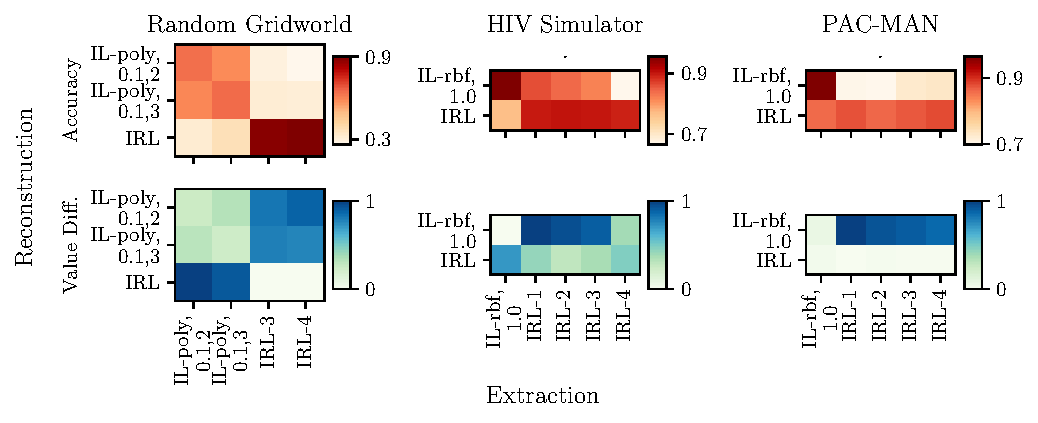
\includegraphics[width=0.75\linewidth]{figures/performance_table.pdf}
\caption{Accuracy (higher is better) and 0-1 scaled value differences (lower is better) averaged over 75 random restarts of every reconstruction model (rows in heatmaps) used for summary extraction with summaries extracted with each model (columns in heatmaps). IRL hyperparameter corresponds to trajectory length; IL hyperparameters indicate kernel, length scale, degree in that order. 
The comparatively high accuracy and low value differences for the reconstructions where the summarization model matches the reconstruction model, indicate that matching the summarization model to the reconstruction model is important for producing a high quality reconstruction.}
\label{fig:computationalResults}
\vspace{-0.2cm}
\end{figure*}

\paragraph{Different reconstruction models result in higher absolute quality reconstructions in different domains when summaries are optimized for them.} The first question we considered was whether one approach---IL or IRL---always produced better summaries. In the HIV simulator and PAC-MAN domains, the IL reconstructions with IL summaries have higher accuracy than the IRL reconstructions with IRL summaries. In the HIV simulator domain, this is reflected in the value difference results, while in the PAC-MAN domain, the methods perform similarly with respect to value difference. In the random gridworld domain, the IRL reconstruction with the corresponding IRL summary has a higher accuracy and lower value difference than IL reconstructions with the corresponding IL summaries. These results indicate that different reconstruction models are more effective in different domains (given a summary optimized for that model). This effect likely has to do with how well each computational model can capture the policy. In the random gridworld, for example, the IRL model can perfectly model the policy but the IL model lacks important spatial information. 

\paragraph{Matching the extraction model to the reconstruction model is the most effective strategy for producing high-quality reconstructions.} Highest quality reconstructions occur when the same model is used for summary extraction and policy reconstruction. This is true even when a particular reconstruction model was generally more accurate. There are two exceptions to this: the IRL reconstruction with IL summary in PAC-MAN, that performs comparably in accuracy and value difference to the IRL reconstruction with IRL summary, and the value difference for the IL reconstruction with the IRL length 4 summary in HIV which is low even though action prediction accuracy is low. In both these cases, the reconstruction quality is no worse than with the summary based on the matched reconstruction model, and in the other cases it is much better. These results indicate that both the IL and IRL summarization methods are effective when the reconstruction model is known, and that using the correct reconstruction model during summarization can be very important for policy reconstruction quality.

\section{Human-Subject Study}

We conducted a human-subject study to test if the findings from our computational simulations generalize to humans, and to examine which reconstruction models people will naturally deploy.

\subsection{Empirical Methodology}

\paragraph{Task.} Participants inspected a summary of an agent's policy, based on which they were asked to predict the agent's actions in a subset of states not included in the summary. This parallels the accuracy measure of reconstruction quality used in the computational experiments, and tests how well people can generalize an agent's behavior from a summary of its policy.

\textit{Domains.} We used the HIV simulator and random gridworld domains because we expected people to have fewer priors about these than PAC-MAN (we disguised the disease, medication and biomarker names for HIV), and because understanding the transition function is more complex in the HIV domain, which we hypothesized would reduce people's ability to use IRL.

\textit{Summaries.} For each domain, we chose one summary each for IL and IRL where the pattern of higher accuracy for matched-summary reconstructions from the computational experiments was maintained. For gridworld, we showed length 24 summaries (IL: polynomial kernel, length scale=0.1, degree=2; IRL: trajectory length=4). For HIV, we showed length 12 summaries (IL: RBF kernel, length scale=1.0; trajectory length=3).\footnote{The HIV summaries are shorter than in the computational experiments so that they will fit on a single page, but this does not affect the trends from the computational results.}

\textit{Prediction States.} We selected test states to satisfy 2 criteria: 1) A similar computational accuracy grid to the full set of unseen states. 2) A uniform distribution over actions taken by the policy. For the random gridworld we selected states that do not have multiple optimal actions in the policy to avoid ambiguity. We describe additional subtleties in \cite{lage2019policysummarization} Appendix C.
 
\paragraph{Design.} Our experiment used a 2X2 between subject design with domain [HIV or gridworld] and summary type [IRL or IL] as the main factors.

\paragraph{Participants.} 147 participants (Gridworld: IL=36, IRL=39; HIV: IL=37, IRL=35) were recruited through Amazon Mechanical Turk (65 female, Mean age = 36.38). 
Participants received a base payment of \$1.5, and a bonus of up to \$1 based on their performance.\footnote{The study was approved by our IRB.}

\begin{figure}[h]
\centering
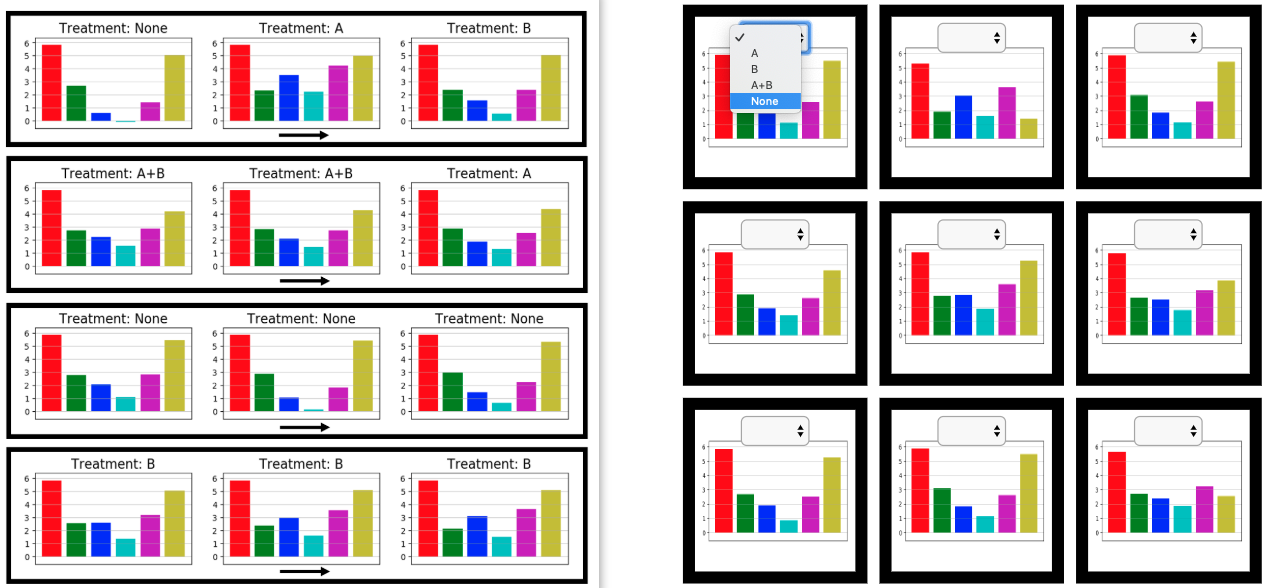
\includegraphics[width=1\columnwidth]{figures/screenshot_hiv_irl.png}
\caption{The user study interface for an IRL summary in the HIV simulator domain. The left side shows the summary and the right side shows the prediction states.}
\label{fig:interface}
\vspace{-0.3cm}
\end{figure}

\paragraph{Interface.} Participants completed all predictions on the same page by choosing actions from dropdown menus with the summary displayed on the left. For the HIV simulator, this consisted of either a grid of independent states each outlined in black for IL, or a grid of trajectories outlined in black for IRL. States were visualized as bar graphs with the action written above (see Figure~\ref{fig:interface}). For the random gridworld, this consisted of the full grid\footnote{We argue this difference is a feature of the domains since it is not obvious how to display the full domain for HIV.}, with actions represented as arrows, and trajectories represented by different colors. See \cite{lage2019policysummarization} Appendix D for screenshots of all task interfaces.

\paragraph{Procedure.} 
Participants were given instructions explaining the domain and task, then a comprehension quiz. Upon passing the quiz, they were shown the summary and answered a practice round predicting 3 actions. Then, they completed the main task and predicted 9 additional actions. After making all predictions, participants were asked to provide a brief text description of how they made their predictions.

\subsection{Results}
\paragraph{In the HIV domain, most people employed IL-based reconstruction models, and performance was better with IL summaries.} Based on the qualitative responses to how people made their predictions, 1 study author coded participants as doing IL, IRL or not obviously doing either and a second author verified the coding (\cite{lage2019policysummarization} Appendix E). In this domain, 78\% of participants reported using IL-based methods for reconstruction (e.g. ``I chose based on the similarity of the blood tests levels from the scenarios on the left''), while only one participant reported using an IRL-based method (``Treatment A is used to decrease middle ones(blue, light blue and purple)...''). Participants who were shown the IL summary performed significantly better compared to those shown the IRL summary with mean accuracy of 0.45 for participants shown an IL summary and 0.33 for those shown an IRL summary (Mann–Whitney U=330.0, n1=37 , n2=35, $P<0.001$ two-tailed). This demonstrates that (1) there are cases where people use IL-based reconstruction models; and (2) matching the computational model used during summarization to people's reconstruction model can improve reconstruction quality, paralleling our simulation results.

\paragraph{In the gridworld domain, people varied in the reconstruction models they employed showing a tendency towards IRL, and there was no difference in performance for different summary types.} In the random gridworld domain, 15\% of participants described IL-based reconstruction (e.g. ``I tried comparing the colors and deciding which was more frequent for a color.''), while 27\% provided descriptions suggesting IRL-based reconstruction (e.g. ``I decided that the computer seems to be always working towards a blue square. I chose the simplest path to get to a blue square''). The remainder of descriptions were too vague to imply a specific method. In contrast to the computational experiments, in this domain there was no significant difference in participants' performance based on summary type with mean accuracy of 0.38 for participants shown an IL summary and 0.37 for those shown an IRL summary (Mann–Whitney U=636.5, n1=36 , n2=37, P=0.24 two-tailed). Participants who reported using IRL reconstruction did perform significantly better than those who did not with mean accuracy of 0.27 for participants who mentioned using IL reconstruction and 0.66 for those who mentioned using an IRL reconstruction (Mann–Whitney U=188.0, n1=11, n2=20, $P<0.001$ two-tailed) as predicted by the computational results, but there was again no difference in performance between summaries among those who used IRL reconstruction. 

\paragraph{There are important differences between computational and human reconstructions including different feature spaces and lower accuracies.} Overall, participants' reconstruction accuracy was lower than predicted by matching the extraction and reconstruction models in the computational simulations, though much higher than random guessing (HIV: 0.33-0.45 compared to 0.67-0.78 for matched and 0.25 for random; Gridworld: 0.37-0.38 compared to to 0.78-1 for matched and 0.2 for random). In the random gridworld domain, reconstruction accuracies were also higher than predicted by mis-matched extraction and reconstruction models (0.37-0.38 compared to 0.11-0.22 for mis-matched). In the qualitative responses for the gridworld condition, some participants described the agent's behavior as based on absolute position (e.g. ``It seems like the agent is trying to get to the center of the screen''), despite being told the agent navigates only based on tile color. In HIV, some people relied on absolute values of the features, and others tried matching the ``shape'' of the bar graphs (e.g. ``I compared the levels of each of the colors and the shapes of the graphs.'') Perhaps due to these disconnects in feature spaces and possible cognitive limitations, people had worse reconstruction accuracy than the computational models with matched summaries; however, these tendencies may have also enabled the better accuracies we observed in the random gridworld domain with mismatched summaries. 

\section{Discussion \& Future Work} 

In this paper, we explored how the computational models of users employed during policy summarization affect people's ability to reconstruct an agent's policy. Computational simulations in 3 diverse domains showed the importance of matching the summarization model to the reconstruction model. Human-subject studies showed that people use different models when reconstructing policies, sometimes deploying IL and sometimes IRL, and that the model used during summarization sometimes affected the quality of their reconstructions. Together, these findings demonstrate the importance of personalizing user models for summarization to domain context.

Our findings suggest several avenues for future work. First, future studies can explore in which circumstances people use different reconstruction models. We hypothesize that familiarity with the domain might be one aspect, as we observed that in the less familiar domain of HIV treatment, people tended toward IL. Better understanding of when people use which approach can help ensure that matching models will be used for extraction and reconstruction.

Second, there are additional nuances to people's extrapolation beyond the choice of IL or IRL -- e.g., which feature representation they use, and how exactly they perform inference. Given the sensitivity of the ability to reconstruct policies to summary extraction models, and the finding that different people use different models even within the same domain, we argue that human-in-the-loop approaches to summary extraction are a promising approach to ensure that summaries match the user's reasoning about a particular domain.

Finally, approaches to policy summarization based on models of user extrapolation can be integrated with those based on ``important'' states or identifying blind-spots. All of these can then be combined with approaches for \emph{explaining} specific agent decisions, to produce summaries that simultaneously demonstrate global agent behavior and explain specific actions. 

\subsubsection{Acknowledgements} 
The authors acknowledge a Google Faculty Research Award and the J.P. Morgan AI Faculty Research Award. IL is supported by NIH 5T32LM012411-02.

\small
\bibliographystyle{named}
\bibliography{bibliography}

\end{document}


